\documentclass[class=report, crop=false, 12pt,a4paper]{standalone}
\usepackage{enumitem}
\usepackage{multicol}
\usepackage{graphicx}
\usepackage{float}
\usepackage{amsmath}
\usepackage{amssymb}
\usepackage{mathtools}
\usepackage{siunitx}
\usepackage{commath}
\usepackage{booktabs}
\usepackage{caption}
\usepackage{array}
\usepackage{ulem}
\usepackage{natbib}
\usepackage[a4paper,width=150mm,top=25mm,bottom=25mm]{geometry}
\setlength{\parindent}{0pt}
\begin{document}
\section{Compressible duct flows}
\subsection{Problem types}
We are concerned with flow in ducts or 'long' pipes whose cross-section area is simple (rectangular / circular / conical). There are three types of problems where:
\begin{enumerate}
    \item changes in cross-sectional area are important ($\dif A \neq 0$).
    \item frictional forces are important (\textbf{momentum is not conserved}) - \textit{Fanno flow} (mass, energy, state).
    \item heating and cooling are important (\textbf{energy is not conserved}) - \textit{Rayleigh flow} (mass, momentum, state).
\end{enumerate}
We study these effects separately and then consider them combined.
\subsection{Influence of changes in cross-section area}
To understand the physics, we simplify the analysis to gas moving without frictional forces and the addition of heat. There are two approaches to analyse the problem:
\begin{enumerate}
    \item Differential approach - how flow properties vary along pipe (Rayleigh flow, Laval nozzle) - sometimes called a 1D model.
    \item Integral approach - relationship between two flow states (Fanno flow, isothermal examples) - sometimes called a 0D model.
\end{enumerate}
We have met these two approaches before:
\begin{enumerate}
    \item Navier-Stokes equation. $$\rho \dfrac{D\underline{u}}{Dt} = - \underline{\nabla} p + \mu \underline{\nabla}^2 \underline{u}$$
    \item Momentum-integral approach. $$\dfrac{\dif}{\dif t} \int_V \left(\rho u\right)\dif V = \int_S \left(-p\underline{I} + \underline{\tau}\right)\cdot \underline{\hat{n}}\dif S$$ Where the integral is taken over a volume $V$ bounded by a surface $S$.
\end{enumerate}
\subsection{Recap of reference states}
The stagnation values are valid for isentropic flows:
\begin{align}
    \dfrac{p}{p_0}       & = \left(1 + \frac{1}{2}\left(\gamma - 1\right)M^2\right)^{-\frac{\gamma}{\gamma - 1}} \\
    \dfrac{\rho}{\rho_0} & = \left(1 + \frac{1}{2}\left(\gamma - 1\right)M^2\right)^{-\frac{\gamma}{\gamma - 1}}
\end{align}
and for adiabatic flows:
\begin{gather}
    \dfrac{T}{T_0} = \left(1 + \frac{1}{2}\left(\gamma - 1\right)M^2\right)^{-1}
\end{gather}
It is important to be aware of what is conserved for adiabatic or isentropic conditions. The reference state of $M = 1$ is useful for flow in pipes where the sonic condition is common. The sonic reference condition is usually referred to as the critical condition and denoted wit ha '*'. Therefore:
\begin{align}
    \dfrac{p_*}{p_0}       & = \left(\frac{1}{2}\left(\gamma - 1\right)M^2\right)^{-\frac{\gamma}{\gamma - 1}} \approx 0.528 \\
    \dfrac{\rho_*}{\rho_0} & = \left(\frac{1}{2}\left(\gamma - 1\right)M^2\right)^{-\frac{\gamma}{\gamma - 1}}  \approx 0.91 \\
    \dfrac{T_*}{T_0}       & = \left(\frac{1}{2}\left(\gamma - 1\right)M^2\right)^{-1} \approx 0.833
\end{align}
In duct flows, the critical state is used. $p_0$, $\rho_0$ are constant when there is no shock. $T_0$ is constant even with a shock.
\subsection{Conservation of mass}
The purpose is to relate $A$ and $M$. The conservation of mass requires (integral or 0D approach and assuming no shocks at the moment):
\begin{gather}
    \dot{m} = \rho u A = \textrm{const} = \rho^* u^* A^*
\end{gather}
or
\begin{gather}
    \frac{\rho}{\rho^*} \frac{u}{u^*} \frac{A}{A^*}
\end{gather}
Substituting for our isentropic and adiabatic parts:
\begin{gather}
    \frac{\rho}{\rho^*} = \left(\frac{1 + \frac{1}{2}\left(\gamma - 1\right)M^2}{\frac{1}{2}\left(\gamma + 1 \right)}\right)^{-\frac{1}{\gamma - 1}}\\
    \frac{u}{u^*} = \frac{M}{M^*} \frac{c}{c^*} = \frac{M}{M^*}\left(\frac{T}{T^*}\right)^{\frac{1}{2}} = M \left(\frac{\frac{1}{2}\left(\gamma + 1\right)}{1 + \frac{1}{2}\left(\gamma - 1\right)M^2}\right)^{\frac{1}{2}}
\end{gather}
THe right-hand side is a constant. It is a state that may, or may not, be realised
\subsection{Relationship between flow state and area}
We are to explore some of the important relationships between the state of the flow and the cross-sectional area.
\begin{figure}[H]
    \centering
    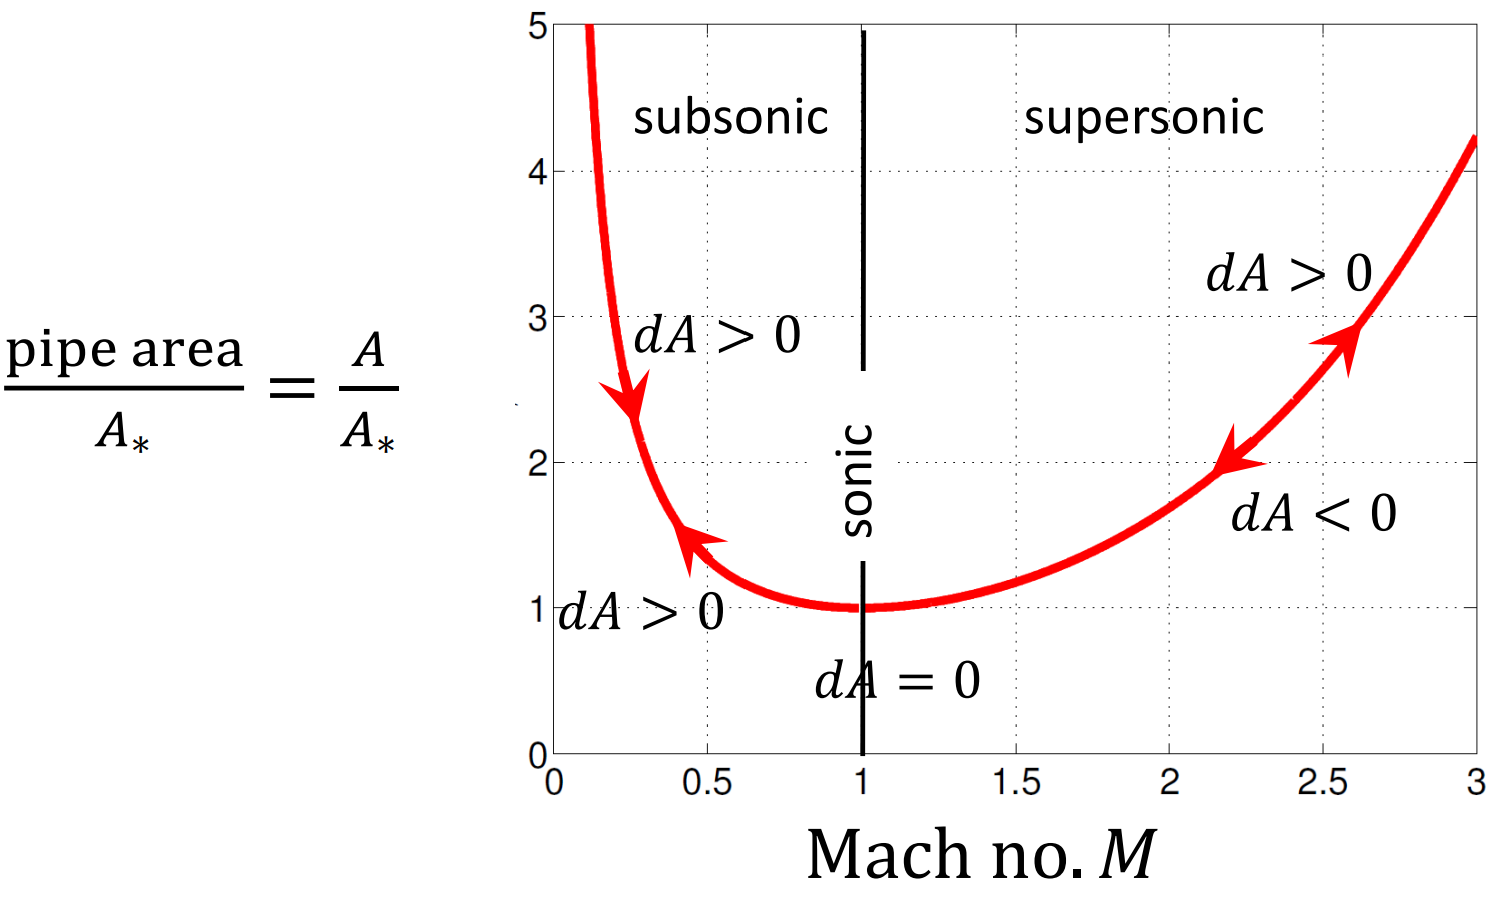
\includegraphics[width = 0.75\textwidth]{../img/diagram52.png}
    \caption{Graph to show pipe area vs Mach number.}
\end{figure}
\begin{table}[H]
    \centering
    \begin{tabular}{@{}llll@{}}
        \toprule
        $\dif A > 0$ & Subsonic   & $\dif M < 0$ & \\
        $\dif A < 0$ & Subsonic   & $\dif M > 0$ & \\
        $\dif A > 0$ & Supersonic & $\dif M > 0$ & \\
        $\dif A < 0$ & Supersonic & $\dif M < 0$ & \\ \bottomrule
    \end{tabular}
    \caption{Table to show pipe area conditions and Mach number}
\end{table}
Profound elements - 2 solutions are possible!
\begin{gather}
    \frac{A}{A^*} = \frac{1}{M}\left(\frac{1+\frac{1}{2}\left(\gamma - 1\right)M^2}{\frac{1}{2}\left(\gamma + 1\right)}\right)^{\frac{\gamma + 1}{2\left(\gamma - 1\right)}}\\
    M = 1 \textrm{ at } \dif A = 0 \textrm{ (point of inflection)}
\end{gather}
\subsection{Creating supersonic flows}
\begin{figure}[H]
    \centering
    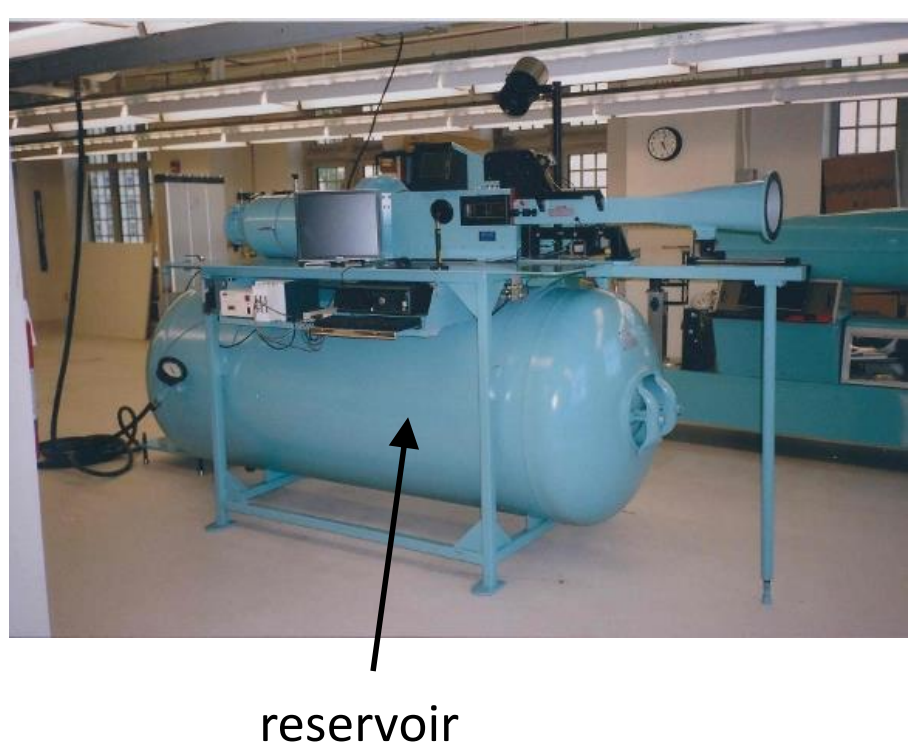
\includegraphics[width = 0.5\textwidth]{../img/diagram53.png}
    \caption{Supersonic flow generator.}
\end{figure}
\begin{figure}[H]
    \centering
    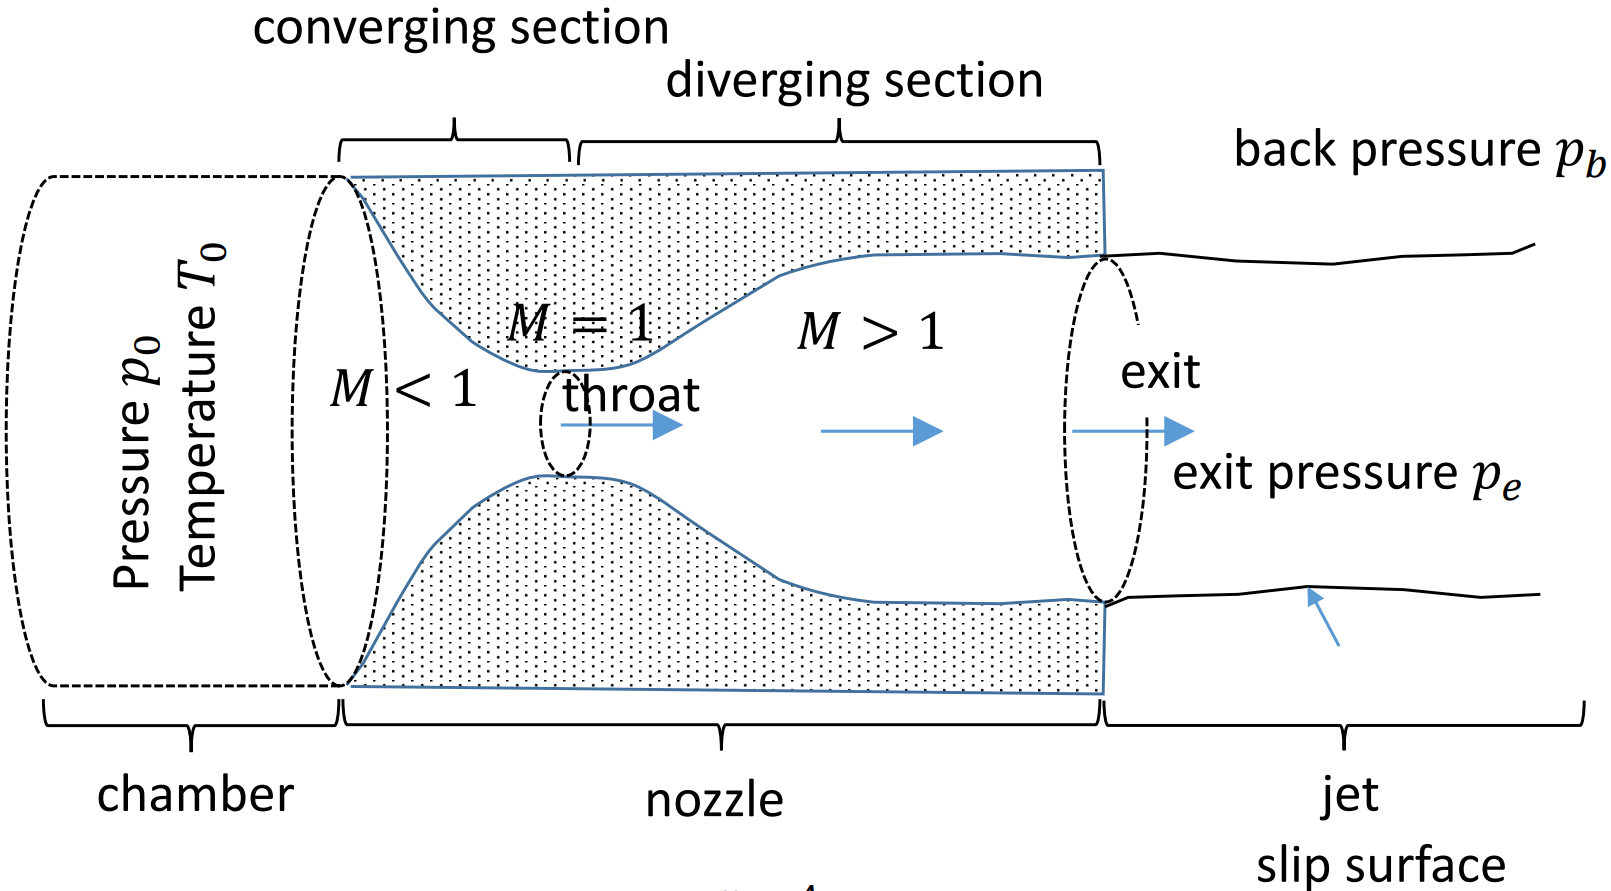
\includegraphics[width = 0.9\textwidth]{../img/diagram54.png}
    \caption{Geometry of supersonic flow generator.}
\end{figure}
This requires a converging, throat and diverging sections. The flow is determined by $\frac{p_b}{p_0}$, $\frac{A_e}{A_t}$.
\subsection{Differential approach to derivation}
Conservation of mass shows:
\begin{gather}
    \rho u A = \textrm{const}
\end{gather}
This can be converted to a differential form:
\begin{gather}
    \log\left(\rho u A\right) = \log \rho + \log u + \log A = \textrm{const}
\end{gather}
Taking the differential gives:
\begin{gather}
    \dfrac{\dif \rho}{\rho} + \dfrac{\dif u }{u} + \dfrac{\dif A}{A} = 0
\end{gather}
Conservation of momentum gives:
\begin{gather}
    \rho u A \dif U = - A \dif p
\end{gather}
For an isentropic flow:
\begin{gather}
    \dfrac{\dif p}{p} = - \gamma \dfrac{\dif \rho}{\rho}
\end{gather}
From the conservation of energy:
\begin{gather}
    \dfrac{T}{T_0} = \left(1 + \dfrac{1}{2}\left(\gamma - 1\right)M^2\right)^{-1}\\
    \dfrac{\dif T}{T} = \dfrac{\frac{1}{2}\left(\gamma -1\right)\dif M^2}{1 + \frac{1}{2}\left(\gamma -1 \right)M^2}
\end{gather}
THis gives:
\begin{gather}
    \dfrac{\dif M^2}{M^2} = -\dfrac{2\left(1 + \frac{1}{2}\left(\gamma - 1\right)M^2\right)}{1-M^2}\dfrac{\dif A}{A}
\end{gather}
Integrate:
\begin{gather}
    \log \frac{A_2}{A_1} = \int_{A_1}^{A_2} \left(\frac{1}{A}\right)\dif A = \int_{M^2_1}^{M^2_2}\left(\frac{1}{M^2}\right)\dif M^2
\end{gather}
This can be manipulated to the formula on the crib sheet.
\subsection{Mass flux relationship}
The mass flux (per unit area) is $\frac{m}{A} = \rho u$. Its derivative w.r.t. $M$ is:
\begin{gather}
    \frac{\dif}{\dif M}\left(\frac{\rho u}{\rho_* u_*}\right) = \left(1-M^2\right)\left(1 + \frac{1}{2}\left(\gamma - 1\right)M^2\right)^{-\frac{\gamma -3}{2\left(\gamma - 1\right)}}\left(\frac{1}{2}\left(\gamma + 1\right)\right)^{\frac{\gamma + 1}{2\left(\gamma -1\right)}}
\end{gather}
The maximum occurs when $M=1$, when the flow is choked. The maximum mass flux is:
\begin{gather}
    \dot{m}_{max} = \rho^* u^* A^* = \left(\frac{1}{\frac{1}{2}\left(\gamma + 1\right)}\right)^{\frac{\gamma + 1}{2\left(\gamma -1\right)}}\left(\frac{\gamma}{RT_0}\right)^{\frac{1}{2}}A^* p_0
\end{gather}
\begin{figure}[H]
    \centering
    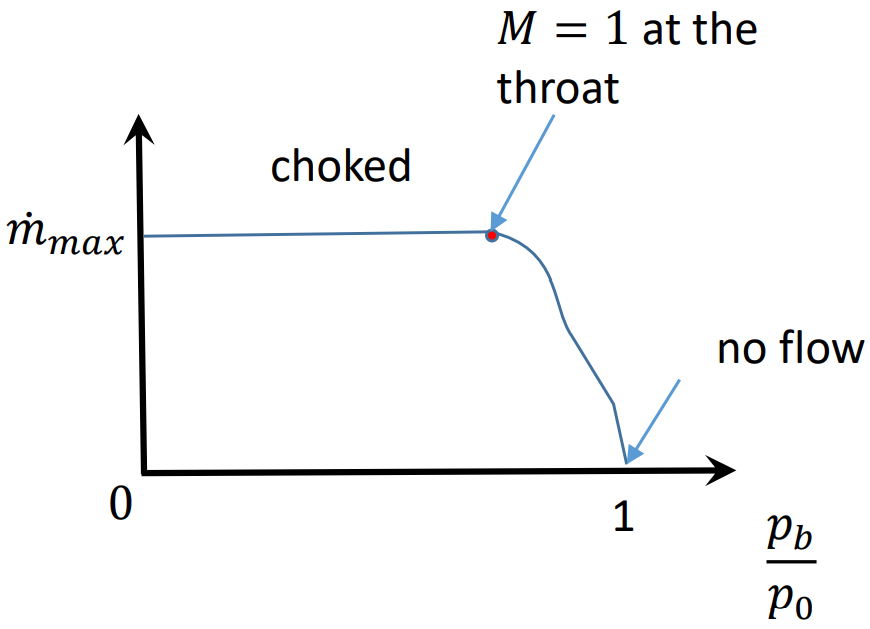
\includegraphics[width = 0.5\textwidth]{../img/diagram55.png}
    \caption{}
\end{figure}
where $p_b$ is the back pressure and $p_0$ is the reservoir pressure.
\subsection{Types of solution available}
\begin{figure}[H]
    \centering
    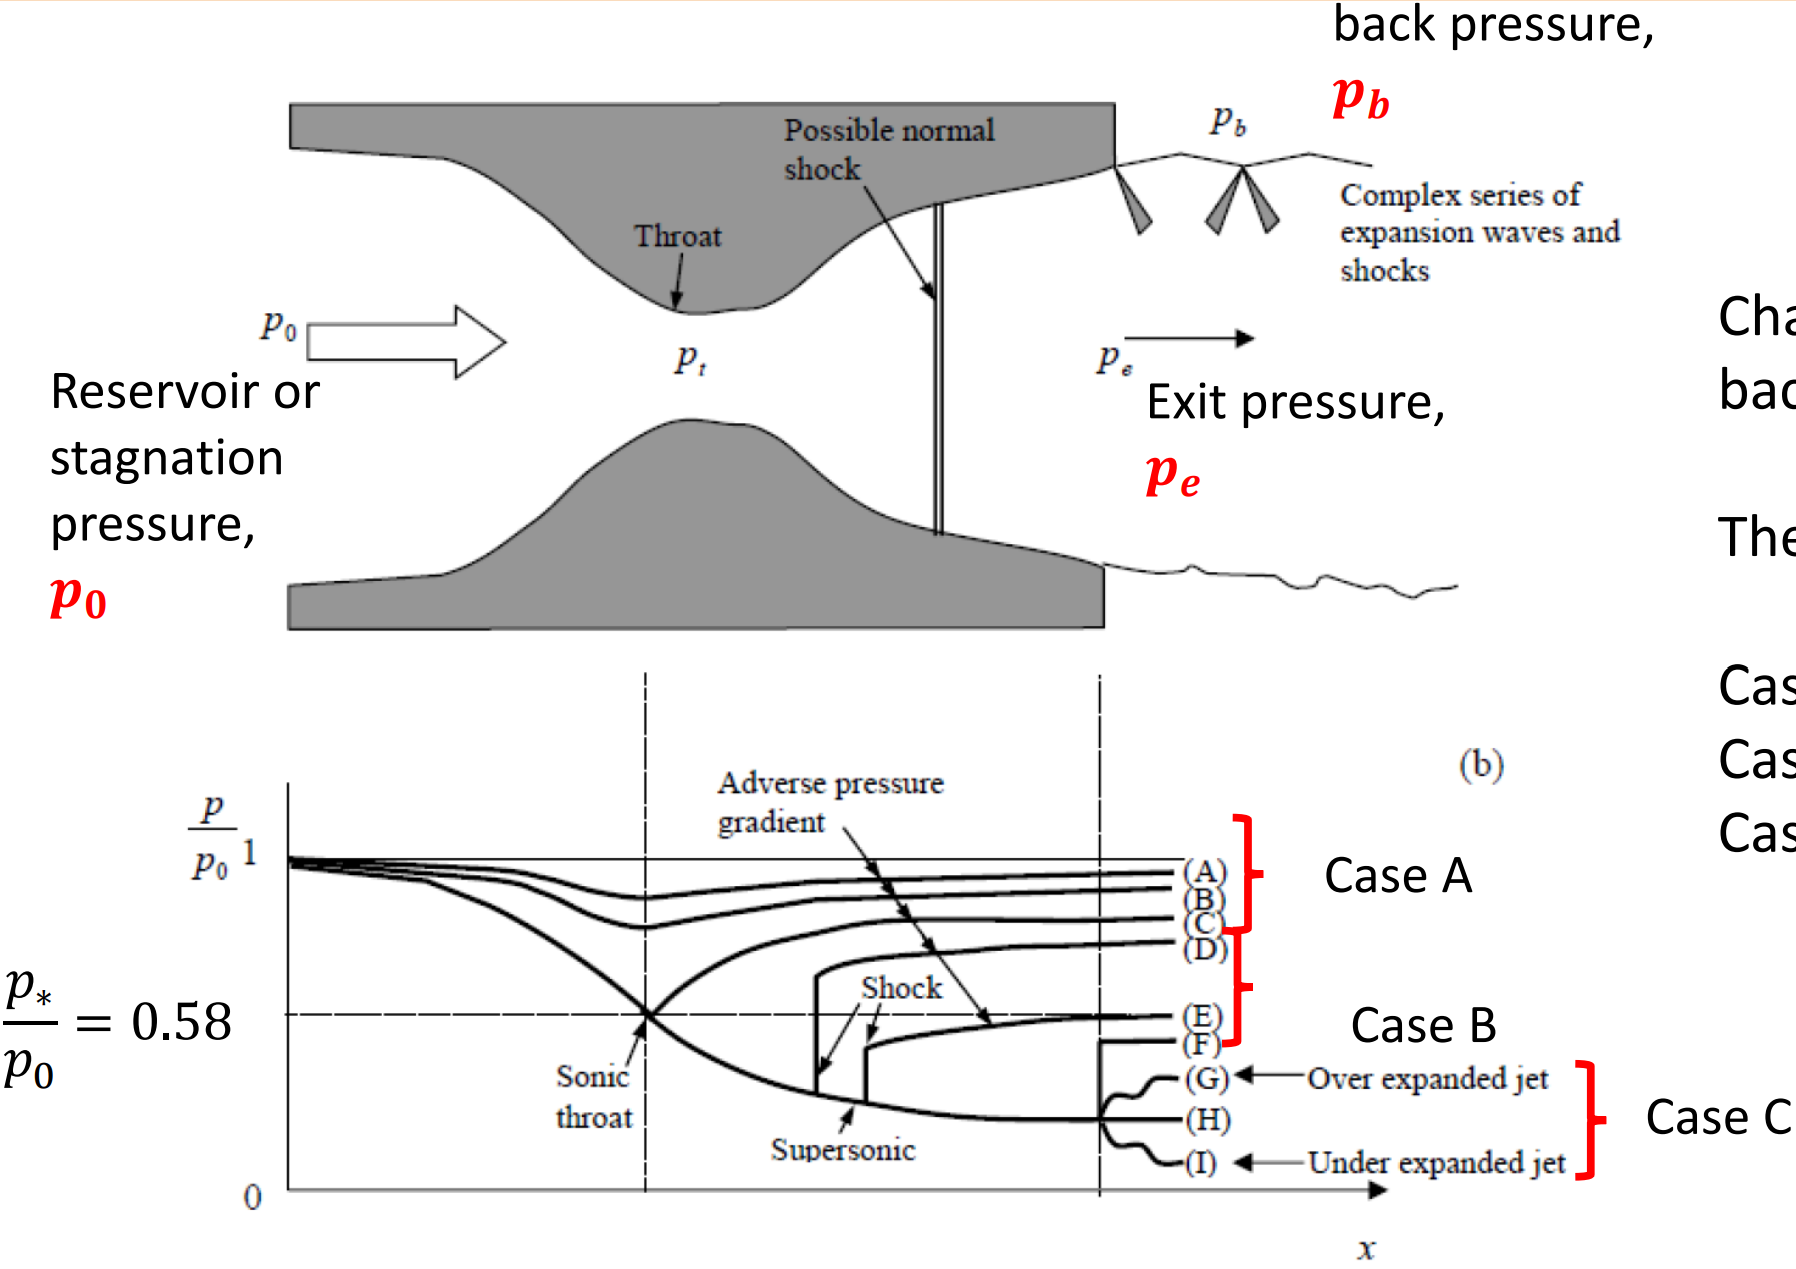
\includegraphics[width = 0.75\textwidth]{../img/diagram56.png}
    \caption{Overview of problem.}
\end{figure}
Characteristics depend on the value of the back pressure. There are three types of solution:
\begin{itemize}
    \item Case A: Subsonic in whole flow ($p_e = p_b$)
    \item Case B: Choked but subsonic outlet ($p_e = p_b$)
    \item Case C: Supersonic outlet ($p_e \leq > p_b$)
\end{itemize}
\subsubsection{Case A: Subsonic flow}
For subsonic flow condition, $M \leq 1$ everywhere and the flow is isentropic because no shocks form. The pressure at the outlet of the duct, $p_e$, is the same as the back pressure, i.e:
\begin{gather}
    p_e = p_b
\end{gather}
The exit Mach number, $M_e$, is determined from the isentropic relationship:
\begin{gather}
    M_e^2 = \frac{2}{\gamma - 1}\left(\left(\frac{p_0}{p_b}\right)^{\frac{\gamma - 1}{\gamma}}-1\right)
\end{gather}
The critical area $A^*$ can be determined from the crib sheet as:
\begin{gather}
    A_* = A_e M_e \left(\dfrac{1 + \frac{1}{2}\left(\gamma - 1\right)M^2_e}{\frac{1}{2}\left(\gamma + 1\right)}\right)^{-\frac{\gamma + 1}{2\left(\gamma -1\right)}}
\end{gather}
The mass flux can be determined at any point along the duct. Choosing the outlet plane, then:
\begin{gather}
    \dot{m} = \rho_e u_e A_e = \rho_0 \sqrt{\gamma RT_0}M_e A_e \left(1 + \frac{1}{2}\left(\gamma - 1\right)M^2_e\right)^{-\frac{\gamma + 1}{2\left(\gamma - 1\right)}}
\end{gather}
This has a maximum value when $\frac{p_b}{p_0} = \frac{p_*}{p_0}$. For a moderate drop in $p_b$ from states A and B, the throat is still subsonic. For curve C, the area ratio is:
\begin{gather}
    \frac{A_e}{A_t} = \frac{A_e}{A_*}
\end{gather}
and the flow is sonic at the throat.
\begin{figure}[H]
    \centering
    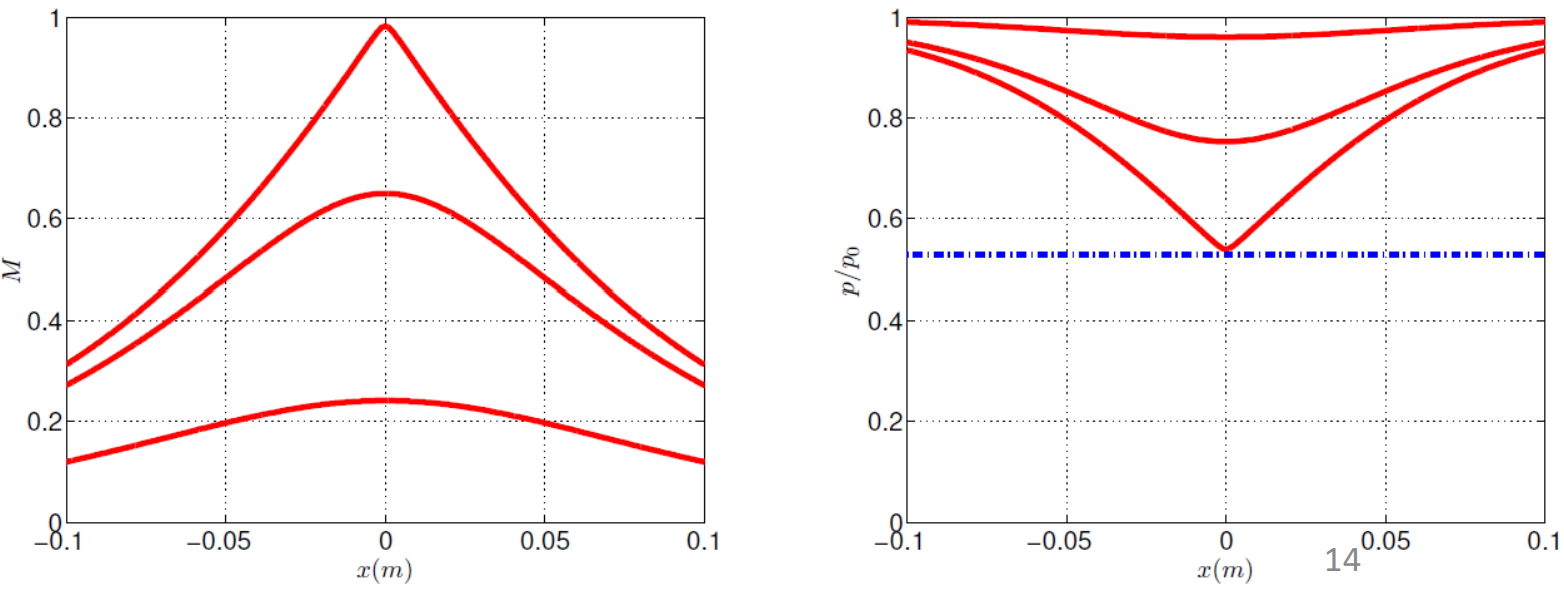
\includegraphics[width = 0.75\textwidth]{../img/diagram57.png}
    \caption{Mach number in the supersonic generator, case A.}
\end{figure}
\subsubsection{Case B: Choked flow with subsonic outlet}
When $p_b$ decreases, the only way for the flow to adapt is for a shock to be created between the nozzle and the outlet. Isentropic model still applies but supplement by normal shock relationship across the shock. If $p_b < p_*$, the nozzle cannot respond because it is choked at its maximum throat mass flow. The flow switches to the supersonic condition after the throat since the flow is mass constrained. The flow passes smoothly through this transition. The only way of the pressure recovering to match the back pressure is to have a normal shock at some location in the nozzle. The exit's jets is then subsonic and is able to match the back pressure.
\begin{figure}[H]
    \centering
    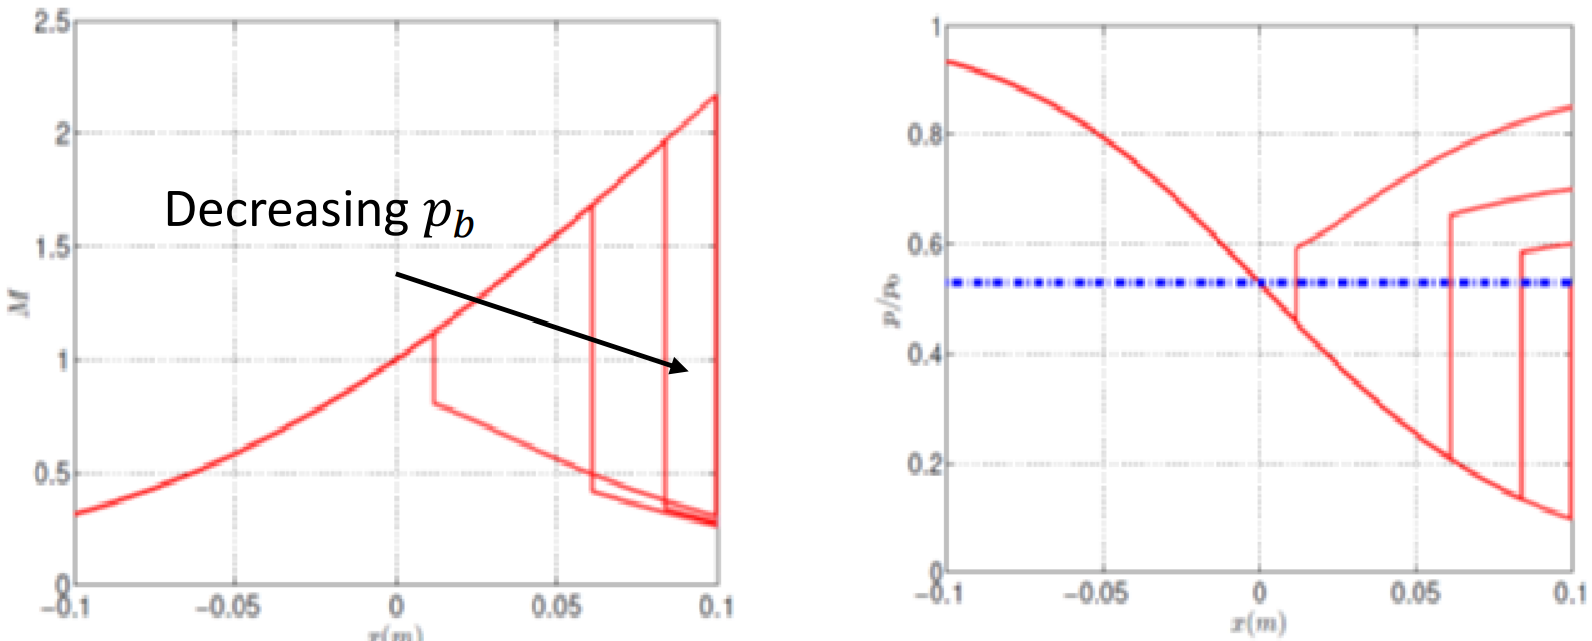
\includegraphics[width = 0.8\textwidth]{../img/diagram58.png}
    \caption{Mach number in supersonic generator, case B.}
    \label{casebmachnumber}
\end{figure}
\ref{casebmachnumber} with subsonic outlet with choked flow and $\frac{p_b}{p_0} =$ 0.53, 0.60, 0.70 and 0.85. Note that $\frac{p_*}{p_0} = 0.528$. After the shock $A_*$ is different before and after the shock ($A_* = A_t$ before the shock.)

The flow characteristics are separated into three parts:
\begin{enumerate}
    \item Choked flow to normal shock.

          In this region, since the flow is choked, $A_* = A_t$. The change in Mach number and pressure are:
          \begin{gather}
              \frac{A}{A_t} = \frac{1}{M}\left(\dfrac{1 + \frac{1}{2}\left(\gamma - 1\right)M^2}{\frac{1}{2}\left(\gamma + 1\right)}\right)^{\frac{\gamma + 1}{2\left(\gamma -1\right)}}\\
              \frac{p}{p_0} = \left(1 + \frac{1}{2}\left(\gamma -1\right)M^2\right)^{-\frac{\gamma}{\gamma -1}}
          \end{gather}
    \item Normal Shock relationship

          If the normal shock occurs at $x = x_s$ where $M_1 = M(x_s)$ and $p_1 = p(x_s)$, the Mach number and pressure after the shock are:
          \begin{gather}
              M^2_2 = \dfrac{1 + \frac{1}{2}\left(\gamma - 1\right)M^2_1}{\gamma M^2_1 - \frac{1}{2}\left(\gamma - 1\right)}\\
              \frac{p_2}{p_1} = \frac{2\gamma}{\gamma + 1}M^2_1 - \frac{\gamma -1}{\gamma + 1}
          \end{gather}

          The stagnation pressure decreases after the shock and needs to be recalculated:
          \begin{gather}
              p_{20} = p_2 \left(1 + \frac{1}{2}\left(\gamma - 1\right)M^2_2\right)^{\frac{\gamma }{\gamma -1}}
          \end{gather}
          The Mach number at the exit is:
          \begin{gather}
              M^2_e = \frac{2}{\gamma - 1}\left(\left(\frac{p_{20}}{p_e}\right)^{\frac{\gamma -1}{\gamma}}-1\right)
          \end{gather}
          $F$ is required normal shock in the duct exit. At the back pressure $G$ no single normal shock can be the job and so the flow compresses outside the exit in a complex series of oblique shocks until it matches $p_b$. In state $F$:
          \begin{gather}
              \frac{A_e}{A_t} = \frac{1}{M_e}\left(\dfrac{1+ \frac{1}{2}\left(\gamma -1\right)M^2_e}{\frac{1}{2}\left(\gamma + 1\right)}\right)^{\frac{\gamma + 1}{2\left(\gamma - 1\right)}}\\
              p_b = p_2 = p_1 \left(\frac{2\gamma}{\gamma + 1}M^2_e-\frac{\gamma -1}{\gamma + 1}\right)\\
              p_1 = p_e = p_0\left(1 + \frac{1}{2}\left(\gamma - 1\right)M_e\right)^{-\frac{\gamma}{\gamma -1}}
          \end{gather}
\end{enumerate}
\subsubsection{Case C: Supersonic outlet}
The final state does not depend on the shape of the throat:
\begin{gather}
    \frac{A_e}{A_t} = \frac{1}{M_e}\left(\dfrac{1 + \frac{1}{2}\left(\gamma -1\right)M^2_e}{\frac{1}{2}\left(\gamma + 1\right)}\right)^{\frac{\gamma + 1}{2\left(\gamma -1\right)}}\\
    \frac{p_e}{p_0} = \left(1 + \frac{1}{2}\left(\gamma -1\right)M^2_e\right)^{-\frac{\gamma}{\gamma - 1}}
\end{gather}
\begin{table}[H]
    \centering
    \begin{tabular}{@{}lll@{}}
        \toprule
        $p_e = p_b$ & Design pressure     &                           \\ \midrule
        $p_e > p_b$ & Under-expanded flow & Exit pressure higher than \\
                    &                     & back pressure, need       \\
                    &                     & expansion fans to match   \\ & & flow.                                              \\
        $p_e < p_b$ & Over-expanded flow  & Exit pressure less than   \\
                    &                     & back pressure so need     \\ & & shocks to increase \\ & & pressure. \\ \bottomrule
    \end{tabular}
\end{table}
\end{document}